\documentclass[letterpaper]{article}
\usepackage{natbib,alifexi}
\usepackage[utf8]{inputenc}
\usepackage[english]{babel}
\usepackage[colorinlistoftodos,prependcaption,textsize=tiny]{todonotes}


\title{Reinforcement learning approaches to movies recommendation}
\author{Antoine Carpentier$^{1}$, Pierre Gérard$^{2}$ \and Julian Schembri$^2$ \\
\mbox{}\\
$^1$Vrije Universiteit Brussel, Brussels \\
$^2$Université libre de Bruxelles, Brussels \\
antoine.carpentier@vub.ac.be, pierre.gerard@ulb.ac.be, julian.schembri@ulb.ac.be}


\begin{document}
\maketitle

\begin{abstract}
  Blabla.
\end{abstract}

\section{Introduction}

blabla

\section{Methods}

blabla et exemple d'image


\begin{figure}[t]
\begin{center}
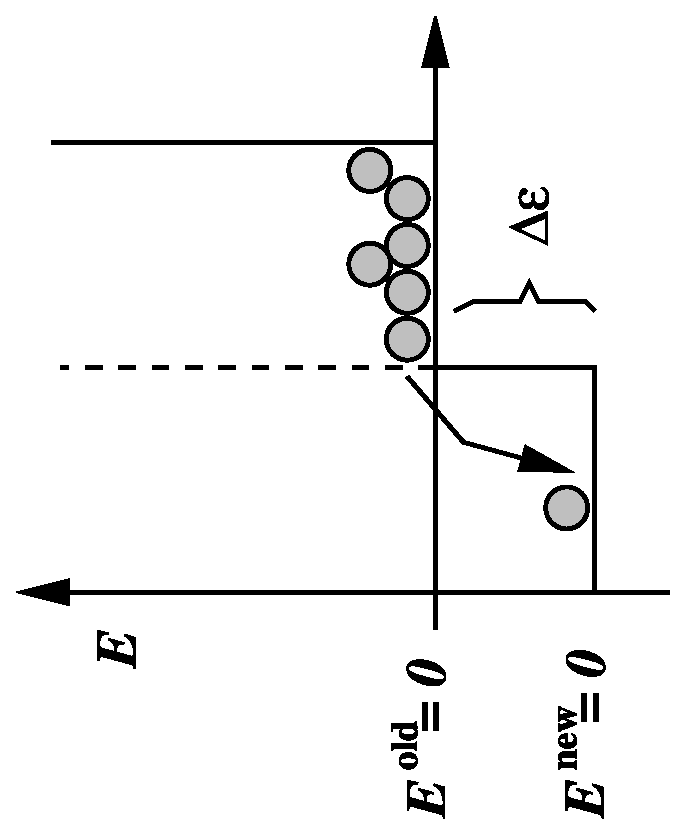
\includegraphics[width=2.1in,angle=-90]{img/fig1.eps}
\caption{``Energies'' (inferiorities) of strings in a first-order
  phase transition with latent heat $\Delta\epsilon$.}
\label{fig1}
\end{center}
\end{figure}


\section{Results}


\section{Discussion}


\section{Acknowledgements}

blabla

\footnotesize
\bibliographystyle{apalike}
\bibliography{biblio}


\end{document}
